\chapter{Methods}
\label{chap:projectdef}



\begin{wrapfigure}{R}{0.3\textwidth}
	\centering
	\includegraphics[width=0.6\textwidth]{Figures/Architecture/Project_framework_diagram}
	\caption{The framework for the system used in this project}
	\label{fig:Project_framework}
\end{wrapfigure}
This project is about learning a car or robot to control and navigate it self. This should be done so the robot don't hit walls or obstacles. to solve this problem, a framework is created, the framework can be seen on \Cref{fig:Project_framework}.

The agent takes information from the environment, in this project the information used as input to the agent is an image. The agent uses the pixels from the image, to process spatial dependencies. The spatial dependencies is found by using of convolutional neural networks (CNN). The output from the CNN is the image features. The image features is used to process the temporal dependencies. To find the temporal dependencies a Recurrent Neural Network (RNN) is used. The RNN used is a special RNN called Long Short Term Memory network (LSTM). When both the spatial and temporal dependencies are found, the state the environment is found. This state is used to build the value function and a policy, which is describe a the Q-network. After the value function and the policy is found, the best suited action to the environment can be determined.


The framework is created with inspiration from the papers  \cite{DBLP:journals/corr/MnihBMGLHSK16} and \cite{Sallab:2017:2470-1173:70}
\newline




%\begin{figure}[H]
%	\centering
% \includegraphics[width=0.3\textwidth]{Figures/ProjectFramework/Project_framework_diagram}
%	\caption{The framework for the system used in this project}
%	\label{fig:Project_framework}
%\end{figure}

\section{Deep Q Networks}
\label{sec:DQN}
The first deep reinforcement learning network there has been created in this project is the Deep Q Network. The Deep Q Network was first time described in the paper "playing Atari with Deep reinforcement learning" \cite{DBLP:journals/corr/MnihKSGAWR13} published by DeepMind. In this paper they learned the computer to play Atari 2600 video games. The computer only observed the screen pixels from the game, and received a reward when the game score increased. The result was remarkable, because the games and the goals in the games are very different. The same architecture was used for seven different games. In 3 of the seven games the computer performed better than the best human. 

To understand the problem the Deep Q Network solved, it is easier to use an example, here we use the game Breakout as an example. In this game you control a paddle at the bottom of the screen, and have to clear the bricks in the top of the screen. This is done by bouncing a ball between the paddle and the bricks. Each time a brick is hit it disappears and the game score increases. The game can be seen on figure \Cref{fig:Atari_breakout}

\begin{figure}[H]
	\centering
	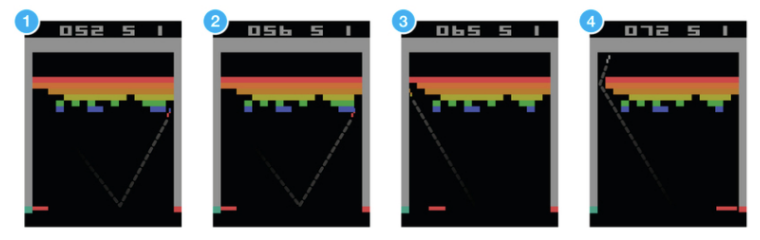
\includegraphics[width=1\textwidth]{Figures/Architecture/DQN/Atari_breakout.png}
	\caption{Atari Breakout game. Image credit: DeepMind\cite{DBLP:journals/corr/MnihKSGAWR13} }
	\label{fig:Atari_breakout}
\end{figure}

To teach a Network how to play this game, the input to the network is the screen images, and the output is the actions of the game: left, right or fire (to launch the ball). One approach to this problem is to treat it as a classification problem - for each screen decide if the paddle should move left, right or press fire. To do this lots of training examples is needed. The problem about this approach is thats really how human learns, we don't need someone to tell us million times which move to choose at each screen. Instead human just need occasional feedback that we did the right thing, and then learn from it ourself. This is the task reinforcement learning tries to solve, more of the reinforcement learning theory can be read in \textbf{Reference to Theory chapter}.

While the idea is quite intuitive, in practice there are numerous challenges. One of the challenges is when hitting a brick and the reward is received, it often has nothing to do with the actions (paddle movement) just before the reward was received. All the work was done when the paddle was positioned correctly and bounced the ball back. This is called the credit assignment problem – i.e., which of the preceding actions was responsible for getting the reward and to what extent.

Another challenge is when a strategy is found and a certain reward is received, should the program stick with that strategy or experiment with something that could lead to a bigger reward. This is called the explore-exploit dilemma – should you exploit the known working strategy or explore other, possibly better strategies. 

The screen pixels obtain most of the relevant information of the game situation, except speed and direction of the ball. This could be covered by having two consecutive screens. 

\subsection{Preprocessing}
The DeepMind paper use preprocessing where the take the last four screen images, resize them to 84x84 and convert to grayscale with 256 gray levels. This will give $256^{84x84x4} \approx 10^{67970}$ possible game states. This will give $10^{67970}$ rows in the imaginary Q-table - more than the number of atoms in the universe. Many pixel combinations never occur, so possible represent it as a sparse table containing only visited states. Most of the states are rarely visited and it would take a lifetime of the universe to the q-table to converge. It should also be possible to have a good guess for Q-values for states we have never seen. 

To do this deep learning comes in to the picture. Neural networks are extremely good at coming up with good features for highly structured data. A way neural networks can be used in reinforcement learning is it could represent the Q-function, where it takes the state (four game screens) and action as an input and output the corresponding Q-value. Another way is to only take game screens as input, and output the Q-value for each possible action. The second approach has the advantages, that if we want to perform a Q-value update or choose the action with the highest Q-value, it can be done by only doing one forward pass in the network and have all Q-values for all possible actions. The two different approaches to use neural network to represent the Q-function can be seen on \Cref{fig:DQN_two_approach}.              


\begin{figure}[H]
	\centering
	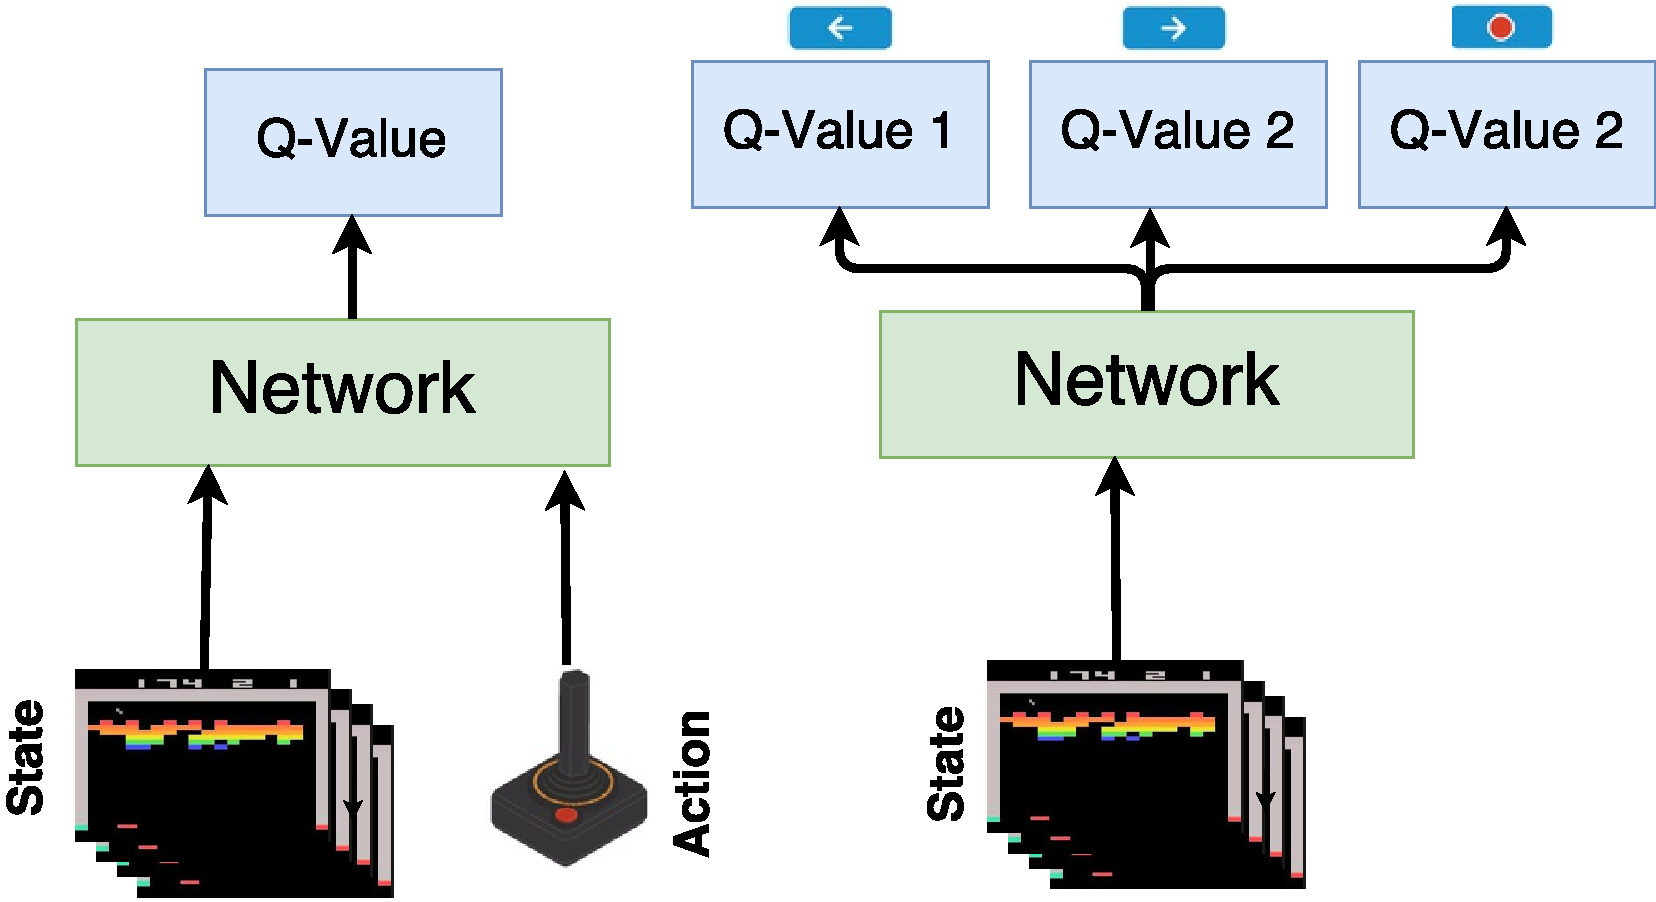
\includegraphics[width=1\textwidth]{Figures/Architecture/DQN/DQN_two_approach.pdf}
	\caption{Left: Naive formulation of deep Q-network. Right: More optimized architecture of deep Q-network, used in DeepMind paper.} 
	\label{fig:DQN_two_approach}
\end{figure}    

\subsection{Network}
The network architecture that DeepMind used can be seen on the table below \Cref{tab:DQN_network}. 

\begin{table}[H]
	\centering
	\caption{Architecture of the Deep Q Network used by DeepMind}
	\label{tab:DQN_network}
	\begin{tabular}{|l|c|c|c|c|c|c|}
		\hline
		\rowcolor[HTML]{9B9B9B} 
		\multicolumn{1}{|c|}{\cellcolor[HTML]{9B9B9B}\textbf{Layer}} & \textbf{Input} & \textbf{Filter size} & \textbf{Stride} & \textbf{Num filters} & \textbf{Activation} & \textbf{Output} \\ \hline
		\cellcolor[HTML]{FFFFFF}\textbf{conv1}                       & 84x84x4        & 8x8                  & 4               & 32                   & ReLU                & 20x20x32        \\ \hline
		\rowcolor[HTML]{C0C0C0} 
		\textbf{conv2}                                               & 20x20x32       & 4x4                  & 2               & 64                   & ReLU                & 9x9x64          \\ \hline
		\cellcolor[HTML]{FFFFFF}\textbf{conv3}                       & 9x9x64         & 3x3                  & 1               & 64                   & ReLU                & 7x7x64          \\ \hline
		\rowcolor[HTML]{C0C0C0} 
		\textbf{fc4}                                                 & 7x7x64         &                      &                 & 512                  & ReLU                & 512             \\ \hline
		\cellcolor[HTML]{FFFFFF}\textbf{fc5}                         & 512            &                      &                 & 18                   & Linear              & 18              \\ \hline
	\end{tabular}
\end{table}

The network can be seen as a classical convolutional neural network with three convolutional layers, followed by two fully connected layers. One of the things which makes this neural network different from the classical neural networks used for image recognition, is no poling layers are used. No pooling layers are used because they buy translation invariance -  the network becomes insensitive to the location of an object in the image. This is okay for image recognition, but for games where the location of the ball is important for deciding the potential reward.  

As seen on \Cref{fig:DQN_two_approach} the input to the network is four 84x84 grayscale game screens. The output of the network are a Q-value for each action, 18 actions for atari games (in breakout there are only 3 actions). The Q-value can be any real number, which make it a regression task. The optimization of the Q-values can be done by a squared error loss. 

\begin{equation}
L=\frac{1}{2}[r+max_{a'}Q(s',a')-Q(s,a)]^2
\end{equation}  

In the squared error loss function is $r+max_{a'}Q(s',a')$ the target, and $Q(s,a)$ is the prediction. Given a transaction <s,a,r,s'>, the Q-table is updated by the following steps:
\begin{enumerate}
	\item Do a feedforward pass for the current state s to get predicted Q-values for all actions.
	\item Do a feedforward pass for the next state s’ and calculate maximum overall network outputs $max_{a'}Q(s',a')$
	\item Set Q-value target for action to $r+max_{a'}Q(s',a')$ (use the max calculated in step 2).For all other actions, set the Q-value target to the same as originally returned from step 1, making the error 0 for those outputs. 
	\item Update the weights using backpropagation.
\end{enumerate}

\subsubsection{Experience Replay}
The approximation of the Q-values using non-linear functions is not very stable. There is many tricks to make i converge. And the problem with this method is it takes long time to converge almost a week on a single GPU. 

The most important tricks is experience replay. During gameplay all the experiences <s, a, r, s’> are stored in a replay memory. While training the network random minibatches are used instead of the recent transition. This breacks the similarity of training samples, and there by avoid the network to reach a local minimum. Experience replay makes the training task more similar to usual supervised learning, which simplifies debugging and testing the algorithm. A way this could be done is by collecting experience from human players, and train on those experiences.
  
\subsubsection{Exploration-Exploitation}
In reinforcement learning the Exploration-Exploitation dilemma, is if the agent should explore or exploit. First when the Q-table or Q-network is initialized randomly, then the prediction of the action is equally random, this is called exploration. As a Q-function converges, it returns more consistent Q-values and the amount of exploration decreases. Q-learning use the exploration as part of the algorithm. But this exploration is “greedy”, it settles with the first effective strategy it finds.

A simple way to do this is to use the $\epsilon$-greedy exploration - with probability $\epsilon$ choose a random action, otherwise go with the “greedy” action with the highest Q-value. DeepMind decreases $\epsilon$ over time from 1 to 0.1. This means in the beginning the system makes random actions to explore the state space maximally, and in the end it settles to a fixed exploration rate.  
        
\section{Deep Deterministic Policy Gradient (DDPG)}
As mentioned in \Cref{sec:DQN} the Deep Q Network solves problems with high-dimensional observation space. But the problem is it can only handle discrete and low-dimensional action space. Many task of interest, most notably physical control tasks, have continuous (real valued) and high dimensional action spaces. The problem with the Deep Q Network is it cannot be applied to continuous domains since it relies on finding the action that maximizes action-value function. In the continuous valued case requires an iterative optimization process at every step. \cite{DBLP:journals/corr/LillicrapHPHETS15}

An obvious approach to adapting the Deep Q Network method to continuous domain is to simply discretize the action space. This have many limitation, most important the curse of dimensionality - the number of actions increases exponentially with the number of degrees of freedom. An example is the human arm is a 7 degrees of freedom system, with a assumption discretization $a_i \sim  \{-k,0,k\}$ for each joint leads to an action space with dimensionality: $3^7 = 2187$. This problem just become bigger with a finer discretion. Such a large action space makes it difficult to explore efficiently. Discretization of action spaces throws away information of the action domain.

The Deep Deterministic Policy Gradient try to solve these problems. The Deep Deterministic Policy Gradient method is a model-free off-policy actor-critic algorithm using deep function approximators that can learn policies in high-dimensional, continuous action space. 

The DDPG algorithm uses some of the some of the deep learning tricks, which was used in the Deep Q Network (DQN) see \Cref{sec:DQN}. To explain more about this algorithm a car simulation environment called "Torcs" is used see \textbf{REF TO TORCS SECTION}. \cite{DDPG_Torcs} 

\subsection{Algorithm}
Even with the DDPG using some of the tricks from the DQN algorithm, it is not straight forward to apply the Q-learning to continuous action space. It is because in continuous action spaces finding a greedy policy requires an optimization of \textit{$a_t$} at every time step - this optimization is too slow to be practical with large, unconstrained function approximators and non trivial action spaces. Here is instead used an actor-critic approach based on the DPG (deterministic policy gradient) algorithm \cite{DBLP:conf/icml/SilverLHDWR14}

The DPG algorithm use a parameterized actor function $\mu(s|\theta^\mu)$ which specifies the current policy by deterministically mapping states to a specific action. The critic $Q(s,a)$ is learned by using the Bellman equation as in Q-learning. The actor is updated by applying the chain rule to the expected return from the start distribution J with respect to the actor parameters:
\begin{equation}
\triangledown_{\theta^\mu} J \approx \mathbb{E}_{s_t \sim \rho^\beta} [\triangledown_{\theta^\mu}Q(s,a|\theta^Q)|_{s=s_t , a=\mu(s_t|\theta^\mu)}]  
\newline
\end{equation}
\begin{equation}
\triangledown_{\theta^\mu} J = \mathbb{E}_{s_t \sim \rho^\beta} [\triangledown_{a}Q(s,a|\theta^Q)|_{s=s_t , a=\mu(s_t)} \triangledown_{\theta_\mu}\mu(s|\theta^\mu)|_{s=s_t} ]
\end{equation} 

This was proved that it is the policy gradient - the gradient of the policy performance. 

Introducing non-linear function approximators means that convergence is no longer guaranteed. The approximators is essential to learn and generalize on large state spaces. The DDPG contribution is to provide modification to DPG inspired of the succes of the DQN, which allow it to use neural networks function approximators to learn in state and action space online. 

One of the challenges of using neural networks for reinforcement learning is that most optimization algorithms assume that the samples are independently  and identically distributed. To solve this problem a replay buffer is used, it is sampling a minibatch uniformly from the buffer - more about the replay buffer see \Cref{sec:DQN}. Because the DDPG is a off-policy algorithm, the replay buffer can be large, allowing the algorithm to benefit from learning across a set of uncorrelated transition.
              
\section{TORCS (The Open Racing Car Simulator)}
\label{sec:TORCS}
The environment to use in reinforcement learning is important, because it is here all the learning will be done. This project is using reinforcement learning in autonomous driving. After reading the post \cite{DDPG_Torcs} that uses TORCS in combination with Gym-TORCS. It was decided that this project will use the same environment, because it seems like it will make a good simulation environment for the task in the project. It is also an environment DeepMind has used to test their algorithms \cite{DBLP:journals/corr/LillicrapHPHETS15} and \cite{DBLP:journals/corr/MnihBMGLHSK16}, it is thereby a well-known environment to use in reinforcement learning. 

The Open Racing Car Simulator or TORCS is a highly portable multi-platform car racing simulation. It is used as ordinary car racing game, as AI racing game and as a research platform. The source code of TORCS is licensed under the GPL ("Open Source") \cite{TORCS_website}. 

Gym-TORCS is a reinforcement learning environment in the TORCS domain. It is made to have an interface which matched Open-AI - A toolkit for developing and comparing reinforcement learning algorithms. It supports teaching agents everything from walking to playing games like Pong or Go \cite{OPENAI_website}. It is smart to match the Open-AI interface because it combines a lot of environment to solve different reinforcement learning tasks. This is done by a simple interface to make it easier to use. \cite{Gym_TORCS_website}. 

Some points why TORCS is useful as an environment for reinforcement learning:
\begin{itemize}
	\item The AI can learn how to drive
	\item It is possible to visualize how the neural networks learn over time and inspect its learning process. Instead of only looking at the final result.
	\item It is easy to visualize when the neural network gets stuck in a local minimum.
	\item Gives an understanding of machine learning technique in automated driving, which is important for autonomous driving technologies 
\end{itemize}

Some pictures from TORCS can be found on \Cref{fig:torcs_screenshots} the below:
\begin{figure} [H]
	\centering
	\begin{subfigure}{.20\textwidth}
		\centering
		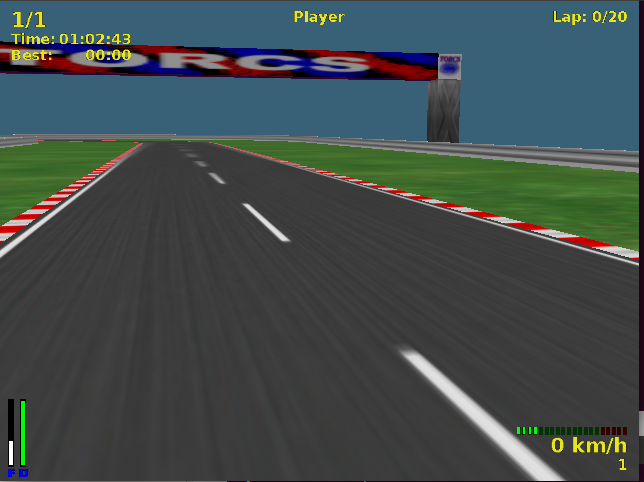
\includegraphics[width=25mm, height=25mm]{Figures/Architecture/Torcs/torcs_2.png}
	\end{subfigure}
	\begin{subfigure}{.20\textwidth}
	\centering
	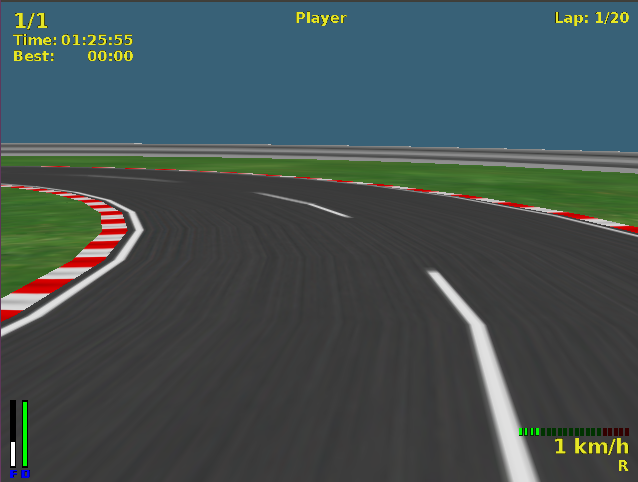
\includegraphics[width=25mm, height=25mm]{Figures/Architecture/Torcs/torcs_3.png}
    \end{subfigure}
	\begin{subfigure}{.20\textwidth}
	\centering
	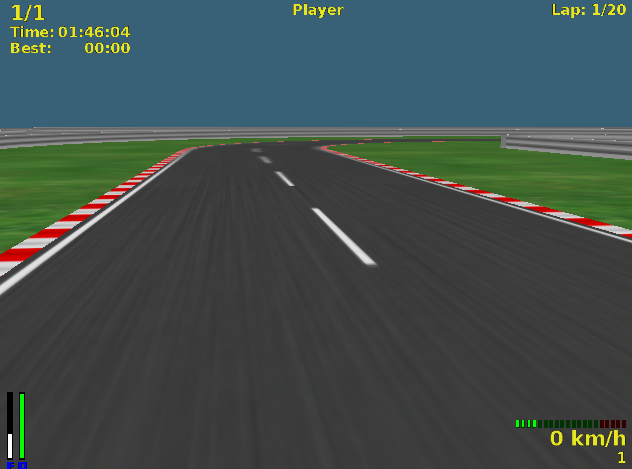
\includegraphics[width=25mm, height=25mm]{Figures/Architecture/Torcs/torcs_4.png}
	\end{subfigure}
	\begin{subfigure}{.20\textwidth}
	\centering
	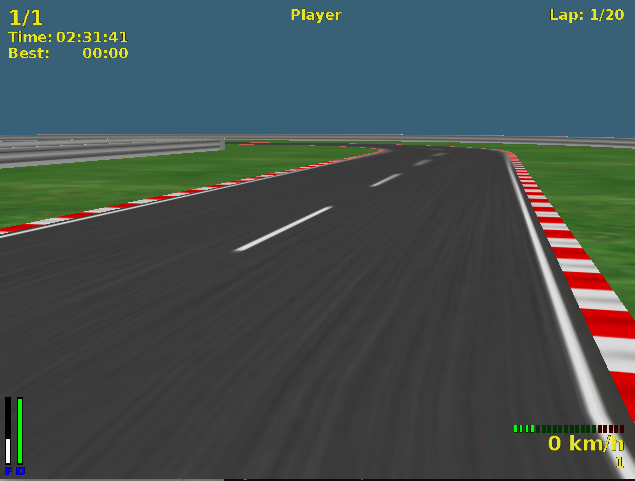
\includegraphics[width=25mm, height=25mm]{Figures/Architecture/Torcs/torcs_5.png}
	\end{subfigure}
	\caption{Screenshots from the TORCS environment}
	\label{fig:torcs_screenshots}
\end{figure}
      
\subsection{Uses in this project}      
The way this environment has been used, is by getting information from the TORCS domain. This information could be the game screen, so the pixels of the game. Another thing the environment has been used for, is to send commands to the game - like steering the car. 

The reinforcement learning should be able to train a network, where the input to the network is the information coming from the game. The output from the network is the determined action, which then will be send to the game. This interaction between the game and the network can be seen on \Cref{fig:TORCS_interaction}.    
 
\begin{figure}[H]
	\centering
	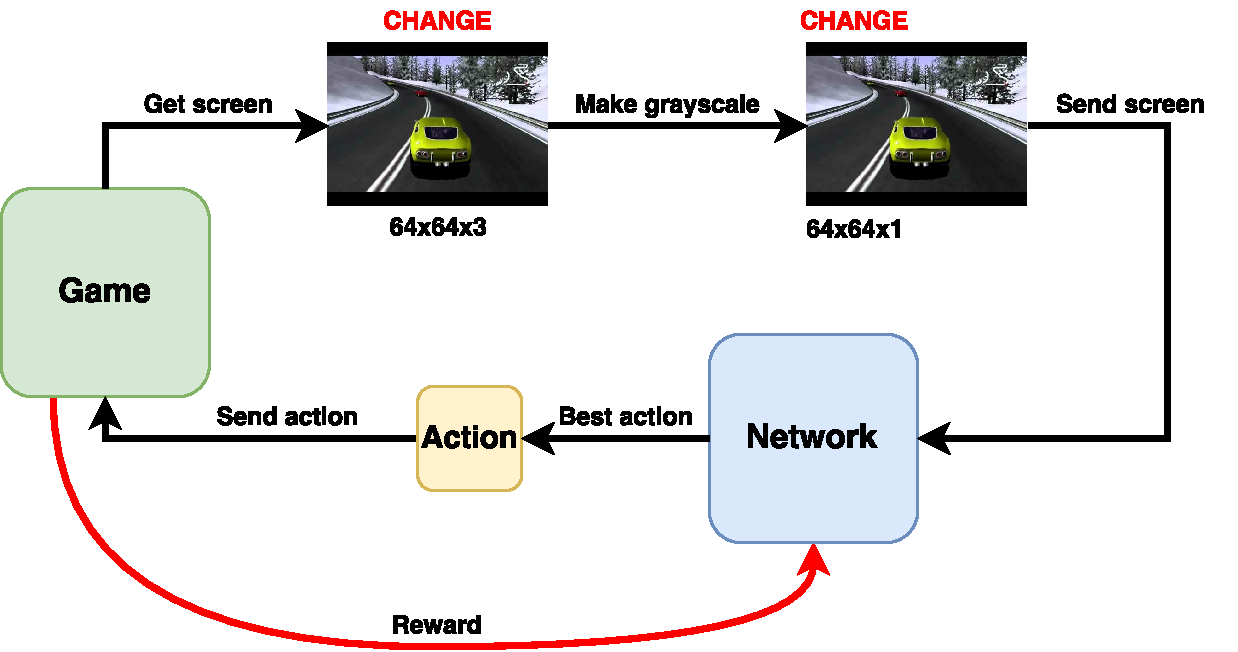
\includegraphics[width=1\textwidth]{Figures/Architecture/TORCS_interaction.pdf}
	\caption{The interaction between the game (TORCS) and the network }
	\label{fig:TORCS_interaction}
\end{figure}

 
As seen on \Cref{fig:TORCS_interaction} the screen is taken from the game, which in this project is TORCS. The screen is the state in our reinforcement learning algorithm. The image screen in this case is of size $64 \times 64$ and have three color channels - red, green and blue. Then some preprocessing is happening for getting this image to the right format, so the network can analyze it. 

 The preprocessing of the image, is to make the image to grayscale. This is done by taken the RGB-image array ($64 \times 64 \times 3$) and separate the 3 color channels red, green and blue. These RGB-values is converted to grayscale values by forming a weighted sum of the R, G and B components:

\begin{equation}
grayscale = 0.2989 \cdot R + 0.5870 \cdot G + 0.1140 \cdot B 
\end{equation}  

The network will then take $64 \times 64 $ image as inputs, more about the network used in this project is described in \Cref{sec:A3C}. The network then uses this input to find the best action, in this state (screen of the game). 

The action the network has found, is then send to the game. The game will then behave after this action and send a reward back to the network. This reward is used to learn the network how to play the game - this is also called training of the network. This procedure continues until the maximum reward is achieved.   
 

 

 
   
\section{Asynchronous Advantage Actor Critic}
The newest breakthrough in RL is the \textit{Asynchronous Advantage Actor Critic} (A3C) approach, and therefore it was chosen to be studied and implemented onto the idea of driver-less cars. In order to achieve a similar environment as the one of a car, and also to be able to get the necessary data easier a car simulator was chosen for the project. Among the existing car simulators encountered in the different online sources, and after analyzing the DDPG implementation on The Open Racing Car Simulator (TORCS) \cite{DDPG_Torcs}, the project settled for this car simulator as well.

The project was mainly inspired from the article \cite{DBLP:journals/corr/MnihBMGLHSK16} summarized in the section \ref{AsyncMeths}, and also from the recent implementation of the A3C into the Doom game elaborated on in \cite{A3CDoom}.

The idea behind the A3C is very much around the same \textit{actor-critic} approach described in the section \ref{PolicyGradMeths}, that more accurately is founded on the presence of both the value function approximator, $\theta_{v}$ and the bootstrapping policy estimator, $\theta$. An additional feature to the actor-critic method is the \textit{asynchronous} part. Instead of having a single agent training on the GPU as in the example of the DDPG project elaborated in the previous section, multiple agents are instantiated for training on different CPU threads simultaneously, and, unlike in the DDPG where there are two different networks, in the A3C the agents share a global network, which is updated as the agents advance. Another new feature of the A3C is the \textit{advantage} element, which is just a mathematical way of expressing how much better some actions ended up to be, and where the estimation should be improved. The update performed by the A3C is of the form $\nabla_{\theta'}\textup{log}\pi(a|s,\theta')A(s,a,\theta,\theta_{v})$, and the formula for the advantage is $\sum_{i=0}^{k-1}\gamma^{i}r_{t+i}+\gamma^kV(s_{t+k},\theta_{v})-V(s_{t},\theta_{v})$, which are both taken from the article \cite{DBLP:journals/corr/MnihBMGLHSK16}. The update formula changes slightly after including the entropy factor in the policy in order to encourage exploration and avoid convergence to an earlier suboptimal solution. The detailed A3C algorithm taken from \cite{DBLP:journals/corr/MnihBMGLHSK16} is listed below.
\begin{algorithm}[H]
	\caption{Asynchronous advantage actor-critic - pseudocode for each actor-learner thread.}
	\label{algo:A3C}
	\begin{algorithmic}
		\State \textit{//Assume global shared parameter vectors $\theta$ and $\theta_{v}$ and counter $T=0$}
		\State \textit{//Assume thread-specific parameter vectors $\theta'$ and $\theta_{v}'$}
		\State Initialize thread step counter $t\leftarrow1$
		\Repeat
		\State Reset gradients: $d\theta\leftarrow 0$ and $d\theta_{v}\leftarrow0$
		\State Synchronize thread-specific parameters $\theta'=\theta$ and $\theta_{v}'=\theta_{v}$
		\State $t_{start}=t$
		\State Get state $s_{t}$
		\Repeat
		\State Perform action $a_{t}$ according to policy $\pi(a_{t}|s_{t}, \theta')$
		\State Receive reward $r_{t}$ and new state $s_{t+1}$
		\State $t\leftarrow t+1$
		\State $T\leftarrow T+1$
		\Until terminal \textbf{or} $t-t_{start}==t_{max}$
		\If {$s_{t}$ is terminal}
		\State $R=0$
		\Else 
		\State $R=V(s_{t},\theta_{v}')$ \textit{//bootstrap from last state }
		\EndIf
		\For {$i \in \left \{ t-1,...,t_{start} \right \}$}
		\State $R\leftarrow r_{i}+\gamma R$
		\State Accumulate gradients wrt $\theta'$:
		\State $d\theta\leftarrow d\theta+\nabla_{\theta'}\textup{log}\pi(a_{i}|s_{i},\theta')(R-V(s_{i},\theta_{v}'))$
		\State Accumulate gradients wrt $\theta_{v}'$:
		\State $d\theta_{v}\leftarrow d\theta_{v} + \partial (R-V(s_{i},\theta_{v}'))^2/ \partial\theta_{v}'$
		\EndFor
		\State Perform asynchronous update of $\theta$ using $d\theta$ and of $\theta_{v}$ using $d\theta_{v}$
		\Until $T>T_{max}$
	\end{algorithmic}
\end{algorithm}

The A3C implementation into the Doom game uses images generated by the vizDoom environment as input data for the well known nonlinear function approximation solution method - ANN. The images become the \textit{states} of the RL problem based on which the AI agent learns to shoot the opponents. The vizDoom environment has a \textit{reward} function predefined, which is triggered when the agent deploys an action in the environment. As the given implementation was made for the \textit{discrete actions space}, the estimated policy or the \textit{actor} provides the probabilities of taking each action in a specific state, and so, in each state the action with the maximal probability is chosen to be pursued. The \textit{critic}, on the other hand, estimates a state-value function for the existing policy and it is used in the composition of the loss function, which represents the performance measure or the \textit{objective function} of the RL problem.

The A3C project developed for the TORCS environment has the same principles as the A3C Doom. It also uses images as the input states into a deep ANN structure and the mathematical model of the problem is similar. The TORCS environment is more flexible and that is an advantage as it offers more freedom for changing things and get better results. For example, it is easier to change the reward function and perform action manipulations, and this will be further explained and illustrated in the next chapter. Another additional implementation is the \textit{continuous} actions space, which is slightly different than the \textit{discrete} actions space implementation; nevertheless they were both preserved in the project for analysis purposes. The structure of the deep ANN will offer more insight on how the program works. Therefore, the overall structure of the ANN of the A3C TORCS project is presented in the following figure:
\begin{figure}[H]
	\centering
	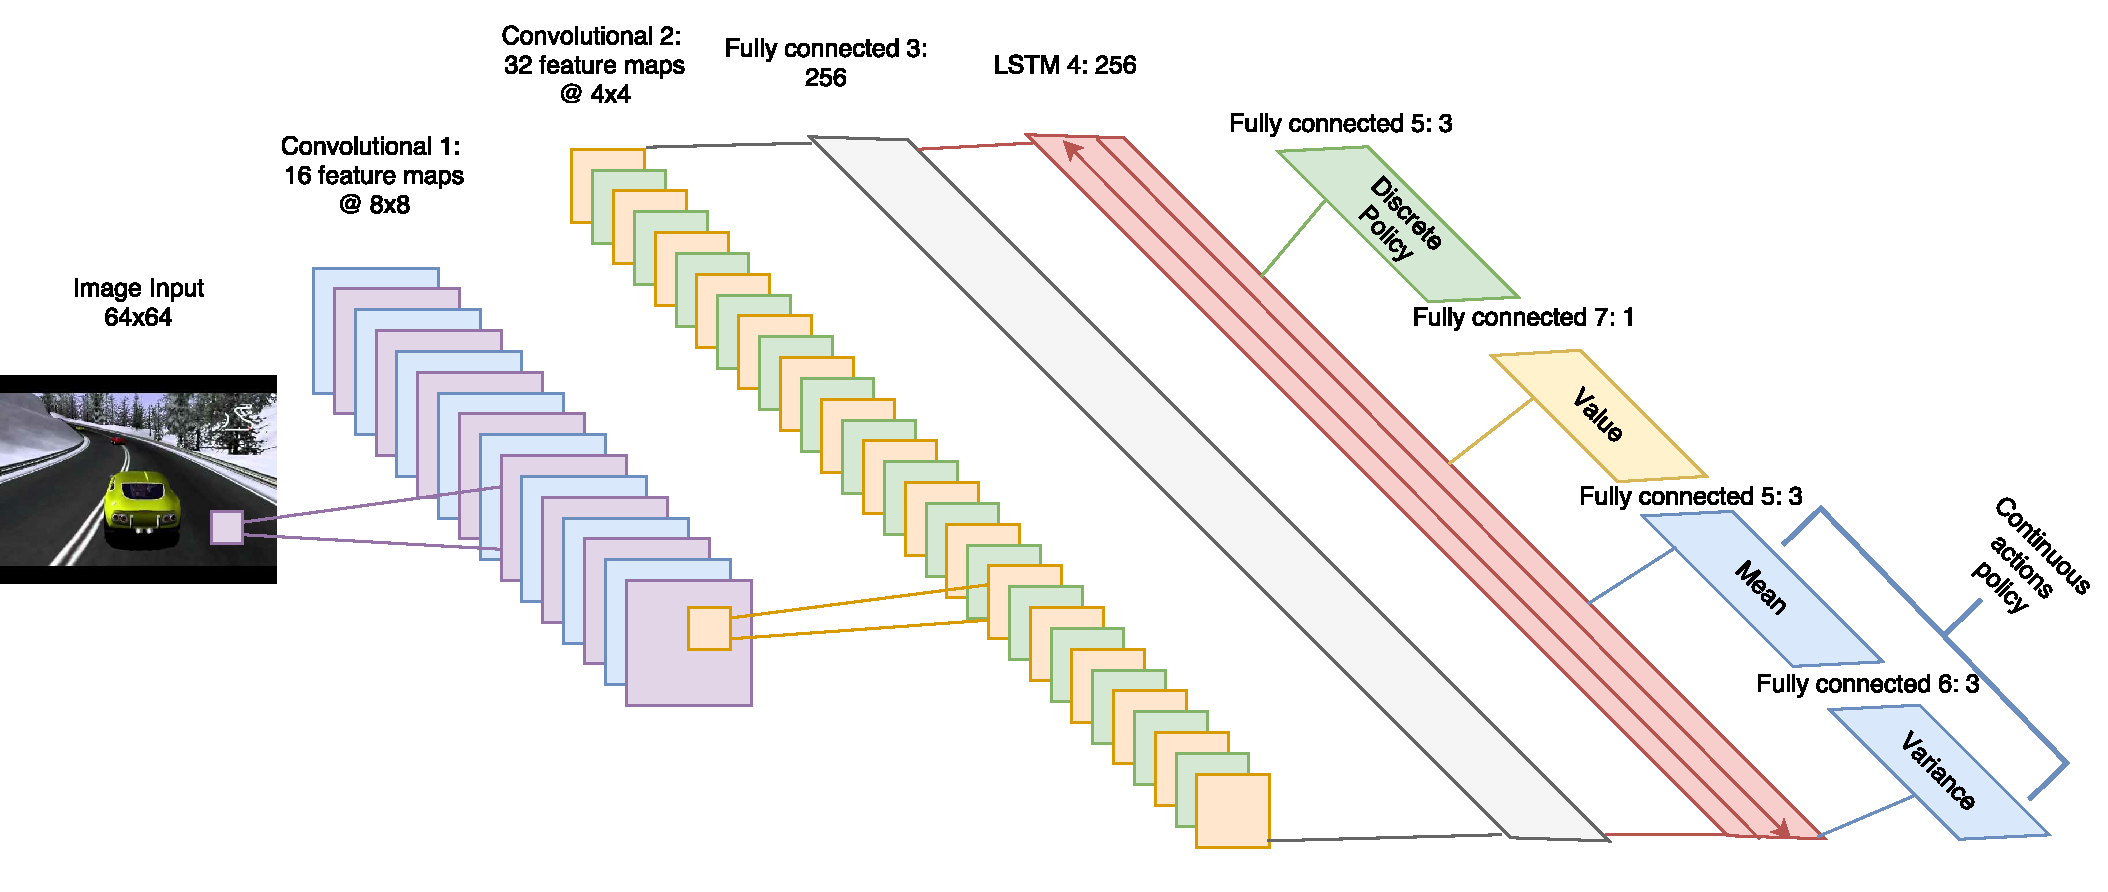
\includegraphics[width=1.25\textwidth]{Figures/A3CTorcs}
	\caption{The ANN structure of the A3C implementation into Torcs}
	\label{A3CTorcs}
\end{figure}
The image of size 64x64 comes into the ANN as input and goes through the first layer of ANN - a convolutional layer that outputs 16 feature maps of sizes 8x8 each. Next, these are again passed through another convolutional layer that outputs 32 feature maps of size 4x4 each, while taking care of spatial correlations. Then the output is flattened with a fully connected layer and passed to a recurrent layer - basic LSTM, that takes care of the temporal dependencies. Finally, the output of the LSTM layer can be used for the last layers of the ANN. The value function is linearly estimated, while the discrete policy is estimated with a softmax activation function and gives the probabilities of each action in the discrete set. For the continuous actions space, on the other hand, the discrete policy is replaced by 2 other layers that estimate the mean $\mu$ and the variance $\sigma$ which form a normal distribution. The formed normal distribution is then sampled to get the action to be passed to the environment.

The flow of the program is as follows. First, a global network is defined and a number of agents or workers are instantiated to train themselves in their own environment using a copy of the global network. During training, as the first state of the environment is received and passed through all the ANN layers, the worker picks the action with the highest probability given by the output of the discrete policy layer, and then the worker executes the action while the environment returns the next state and the reward. The states keep coming during an episode and the rewards keep accumulating together with the values in an episode buffer. At every step the global network is being updated with the data from the episode buffer, and when the buffer is full, then the network bootstraps from the current value estimate to update the whole network. The update of the global network happens by applying gradients that were computed for a defined loss function. A very general illustration of the flow of the program is shown below.
\begin{figure}[H]
	\centering
	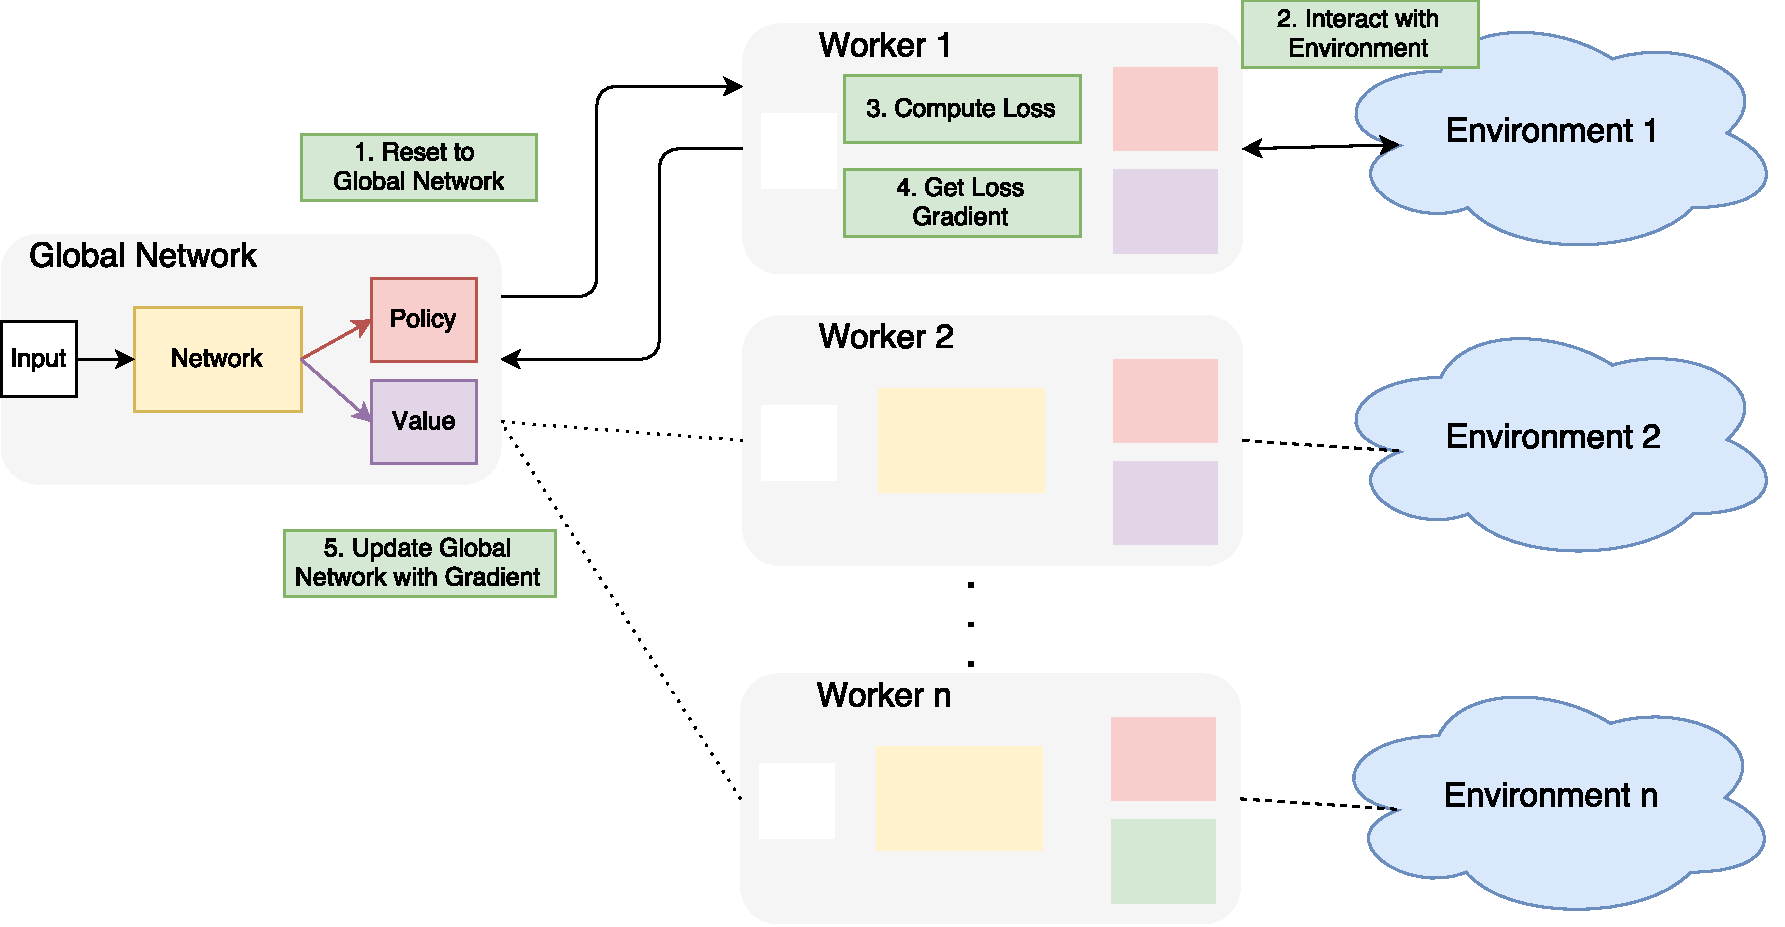
\includegraphics[width=1.25\textwidth]{Figures/Flow}
	\caption{The flow of the A3C Torcs program}
	\label{Flow}
\end{figure}
The loss function is composed of the value loss, policy loss and the entropy loss. Each of these are assigned specific weights that they would have in the total loss result. This loss function represents the performance measure of the problem, the goal, or the objective function. The gradient of the loss function with respect to the weights of the ANN are calculated and applied using an optimizer. The recommended optimizers are RMSProp and, an evolved form of it - the Adam optimizer. The learning rate for these is 1e-4. The discount factor used for the RL problem stated is 0.99.